\setlength{\headheight}{14.49998pt}
\addtolength{\topmargin}{-2.49998pt}

\section{The Abstraction of Mathematical Ideas}

To explain what I mean by \textit{abstraction} - the word that I have used dozens of times by now, I will present three seemingly unrelated ideas in mathematics and demonstrate how they converge into a single concept when thought abstractly.

\subsection{Idea 1: Matrix Multiplication and Permutation Matrices} 

\vspace{3pt} 
The first example comes from the course on \textit{Linear Algebra}. \textit{Have you ever wondered why you multiply two matrices the way you do?} It seems so bizzare that when you are adding two 3 $\times$ 3 matrices, you are adding elementwise; but when you are multiplying them, then suddenly a weird rule of multiplying rows with columns comes into picture. \textit{Why?} \\

I expect you are fami
liar with the facts that columns of a matrix are \textit{vectors} and $n$ simultaneous linear equations with $n$ variables can be written in the matrix form $AX = B$, where $A$ is the $n \times n$ coefficient matrix, $X$ is the $n \times 1$ matrix of unknowns and $B$ is the $n \times 1$ resultant vector. Geometrically, since each column of the coefficient matrix is a vector in $n$ dimensions, if they are \textit{linearly independent}, we will be able to find a solution i.e. a list of linear combination coefficients $X$ such that a linear combination of those vectors in $A$ gets us the resultant vector $B$. \\

By the nature of the visualization itself in the column picture, if we were to find not just a single linear combination that results in $B$, but two more linear combinations that result in vectors $C$ and $D$ too, the equation becomes 

\begin{center}
$A \cdot \begin{bmatrix} X_1 & X_2 & X_3 \end{bmatrix} = \begin{bmatrix} B & C & D \end{bmatrix}$
\end{center}

If you put the appropriate elements in this matrix, and try to write three linear combinations i.e. three sets of simultaneous linear equations, you will see the reason - why we multiply the matrices the way we do so. From this idea, it should also get clear that the multiplication $A.B$ has a different meaning than $B.A$. This implies, matrix multiplication is not commutative.\\

\textit{But why do we care so much about matrix multiplications?} Because we want to understand the impact on a matrix when it is multiplied by another matrix. \\

Now that we know matrix multiplication is a collection of linear combinations \textit{(this idea is further refined to be called as \textbf{linear transformation})}, we can easily confirm that - if $AB = B$, then $A$ should have a form where diagonal elements are 1 and rest are 0. It's the \textit{identity matrix}. \\

Let's do a reverse-engineering exercise. If

\begin{equation}
    E.
    \begin{bmatrix}
        1 & 2 & 1 \\
        3 & 8 & 1 \\
        0 & 4 & 1
    \end{bmatrix}
    =
    \begin{bmatrix}
        1 & 2 & 1 \\
        0 & 2 & -2 \\
        0 & 4 & 1
    \end{bmatrix}
\end{equation}

then what is $E$? \\

From the first look it is clear that $E$ is very close to the identity matrix as only the second row is different. If we sum three negatives of [1 2 1] and one positive of [3 8 1], we will get [0 2 -2]. Hence, 

$$
E =
\begin{bmatrix}
    1 & 0 & 0 \\
    -3 & 1 & 0 \\
    0 & 0 & 1
\end{bmatrix}
$$

Now what if I have to nullify the effect of multiplication of $E$ shown above on $A$? We should add 3 times the first row to the second row, to compensate for subtracting three times the first row from the second. Notice how the elements of the matrix are acting as row-selectors. 

$$
E^{-1} =
\begin{bmatrix}
    1 & 0 & 0 \\
    3 & 1 & 0 \\
    0 & 0 & 1
\end{bmatrix}
$$

And we can confirm that their effects nullify, because $E.E^{-1} = I$. This gives us the concept of \textit{inverses} in matrices. The matrices that you shall encounter will be very complex, but the core principle behind the matrix multiplication remains the same. 

\subsubsection{Permutation Matrices}

Recall, that the matrix equation $AX = B$ is the set of $n$ equations with $n$ variables. The order in which these equations appear should have no impact on the final solution. This implies, that rows can come in any permutation, the final solution remains unchanged. The matrix $P$ whose effect when multiplied on $A$ is to reorder the rows of $A$ is called the \textit{permutation matrix}. \\

In a $3D$ space, there are 6 permutation matrices, as shown below. \\

\[
\begin{bmatrix}
1 & 0 & 0 \\
0 & 1 & 0 \\
0 & 0 & 1
\end{bmatrix}
\hspace{1em}
\begin{bmatrix}
1 & 0 & 0 \\
0 & 0 & 1 \\
0 & 1 & 0
\end{bmatrix}
\hspace{1em}
\begin{bmatrix}
0 & 1 & 0 \\
1 & 0 & 0 \\
0 & 0 & 1
\end{bmatrix}
\hspace{1em}
\begin{bmatrix}
0 & 1 & 0 \\
0 & 0 & 1 \\
1 & 0 & 0
\end{bmatrix}
\hspace{1em}
\begin{bmatrix}
0 & 0 & 1 \\
1 & 0 & 0 \\
0 & 1 & 0
\end{bmatrix}
\hspace{1em}
\begin{bmatrix}
0 & 0 & 1 \\
0 & 1 & 0 \\
1 & 0 & 0
\end{bmatrix}
\] \\

\textit{\textbf{Note:}} The elements of the above set of permutation matrices are representing some sort of \textit{action}. The effect of the \textit{action} is to reorder the rows of the matrix on which the permutation matrix is operated on. To operate any permutation matrix $P$ on $A$, you have to left-multiply $P$ on $A$. 

\subsection{Idea 2: Symmetries of a Triangle}

Imagine we have a shape of a triangle. The question is - \textit{what kind of operations can I perform on this shape?} Clearly, this is a shape. It's not a number on which we can perform addition or multiplication or any such operation which we would define for a number. The only two actions that are possible to perform on this shape are: \textit{rotation} and \textit{reflection}. You can rotate this triangle by some angle or you can flip it. \\

But, \textit{why are we performing these operations? What's our agenda?} The agenda is we want to learn about the symmetries of triangle. Understanding  symmetries involves exploring different ways a triangle can be transformed while preserving its appearance. We will examine how a triangle can be rotated or flipped to match its original position. \\

Consider the triangle \( ABC \) as shown below.

\begin{center}
    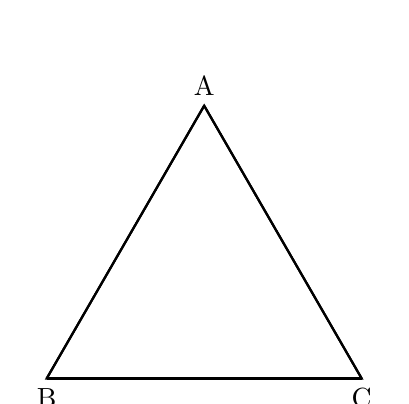
\begin{tikzpicture}
        % Draw the triangle
        \draw[thick] (0,0) -- (4,0) -- (2,3.464) -- cycle;
        
        % Label the vertices
        \node at (0,0) [below] {B};
        \node at (4,0) [below] {C};
        \node at (2,3.464) [above] {A};
        
        % Optionally, draw the sides
        \draw[thick] (0,0) -- (4,0); % AB
        \draw[thick] (4,0) -- (2,3.464); % BC
        \draw[thick] (2,3.464) -- (0,0); % CA
        
        \end{tikzpicture}
\end{center}

\subsubsection{Rotations}

Rotations involve turning the triangle around its center. The triangle can be rotated by angles that are multiples of \( \frac{360^\circ}{3} = 120^\circ \).

\begin{itemize}
    \item \textbf{Rotation by \( 0^\circ \):} This is the identity rotation, where the triangle remains unchanged. This is represented by:
    \[
    \text{Identity: } \text{Triangle} \rightarrow \text{Triangle}
    \]
    
    \item \textbf{Rotation by \( 120^\circ \):} Rotating the triangle by \( 120^\circ \) counterclockwise about its center maps each vertex to the position of the next vertex in a counterclockwise direction. We denote this rotation as \( R_{120^\circ} \). In a triangle with vertices \( A, B, \) and \( C \), the effect is:
    \[
    R_{120^\circ}: A \rightarrow B, \; B \rightarrow C, \; C \rightarrow A
    \]
    
    \item \textbf{Rotation by \( 240^\circ \):} This rotation maps each vertex to the position of the previous vertex in a counterclockwise direction. We denote this rotation as \( R_{240^\circ} \). For vertices \( A, B, \) and \( C \), the effect is:
    \[
    R_{240^\circ}: A \rightarrow C, \; B \rightarrow A, \; C \rightarrow B
    \]
\end{itemize}

\begin{center}
    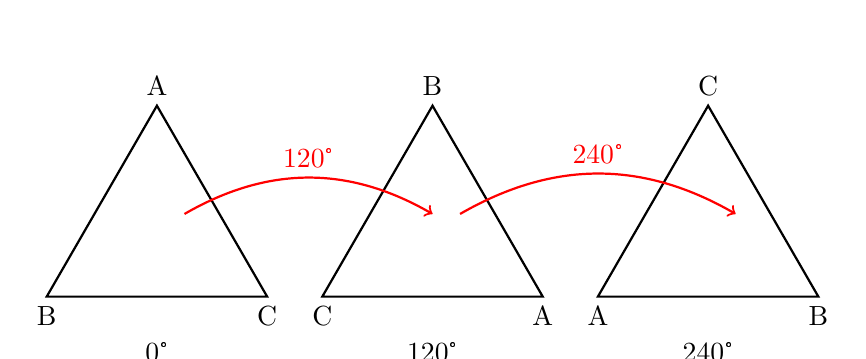
\begin{tikzpicture}[scale=0.7]
        % Original Triangle (0 degrees)
        \begin{scope}[shift={(-5,0)}]
            \draw[thick] (0,0) -- (4,0) -- (2,3.464) -- cycle;
            \node at (0,0) [below] {B};
            \node at (4,0) [below] {C};
            \node at (2,3.464) [above] {A};
            \node at (2,-1) {0°};
        \end{scope}
        
        % Rotated 120 degrees
        \begin{scope}[shift={(0,0)}]
            \draw[thick] (0,0) -- (4,0) -- (2,3.464) -- cycle;
            \node at (0,0) [below] {C};
            \node at (4,0) [below] {A};
            \node at (2,3.464) [above] {B};
            \node at (2,-1) {120°};
        \end{scope}
        
        % Rotated 240 degrees
        \begin{scope}[shift={(5,0)}]
            \draw[thick] (0,0) -- (4,0) -- (2,3.464) -- cycle;
            \node at (0,0) [below] {A};
            \node at (4,0) [below] {B};
            \node at (2,3.464) [above] {C};
            \node at (2,-1) {240°};
        \end{scope}
        
        % Transition arrows between triangles
        \draw[->,thick,red] (-2.5,1.5) to[bend left] node[midway,above] {120°} (2.0,1.5);
        \draw[->,thick,red] (2.5, 1.5) to[bend left] node[midway,above] {240°} (7.5,1.5);
    \end{tikzpicture}
\end{center}

\subsubsection{Reflections}

Reflections involve flipping the triangle over a line of symmetry. A triangle has three lines of symmetry, each passing through a vertex and the midpoint of the opposite side.

\begin{itemize}
    \item \textbf{Reflection over the line through \( A \) and the midpoint of \( BC \):} This reflection maps the triangle to itself by flipping it over the line passing through vertex \( A \) and the midpoint of the side \( BC \). We denote this reflection as \( F_A \):
    \[
    F_A: B \leftrightarrow C, \; A \text{ remains fixed}
    \]
    
    \item \textbf{Reflection over the line through \( B \) and the midpoint of \( AC \):} This reflection maps the triangle to itself by flipping it over the line passing through vertex \( B \) and the midpoint of the side \( AC \). We denote this reflection as \( F_B \):
    \[
    F_B: A \leftrightarrow C, \; B \text{ remains fixed}
    \]
    
    \item \textbf{Reflection over the line through \( C \) and the midpoint of \( AB \):} This reflection maps the triangle to itself by flipping it over the line passing through vertex \( C \) and the midpoint of the side \( AB \). We denote this reflection as \( F_C \):
    \[
    F_C: A \leftrightarrow B, \; C \text{ remains fixed}
    \]
\end{itemize}

\begin{center}
    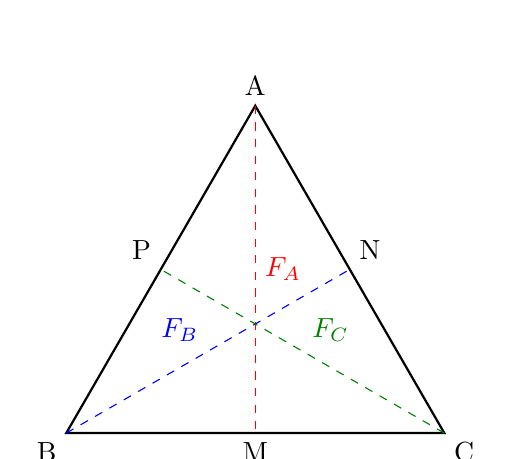
\begin{tikzpicture}[scale=1.2]
        % Define coordinates
        \coordinate (A) at (0,3.464);
        \coordinate (B) at (-2,0);
        \coordinate (C) at (2,0);
        
        % Draw the main triangle
        \draw[thick] (A) -- (B) -- (C) -- cycle;
        
        % Label vertices
        \node[above] at (A) {A};
        \node[below left] at (B) {B};
        \node[below right] at (C) {C};
        
        % Draw and label perpendicular bisectors
        \draw[red, dashed] (A) -- (0,0) node[midway, right] {$F_A$};
        \draw[blue, dashed] (B) -- (1,1.732) node[midway, above left] {$F_B$};
        \draw[green!50!black, dashed] (C) -- (-1,1.732) node[midway, above right] {$F_C$};
        
        % Label midpoints
        \node[below] at (0,0) {M};
        \node[above right] at (1,1.732) {N};
        \node[above left] at (-1,1.732) {P};
    \end{tikzpicture}
\end{center}

Now, it's evident that three rotations in sequence or two flips along the same line of symmetry cancel out as they bring the original configuration of the triangle back. \textit{How many different configurations are possible?} \textbf{Six!} The six configurations of the triangle are: \{$ABC$, $ACB$, $BAC$, $BCA$, $CAB$, $CBA$\}. Honestly, we don't care much about the configuration of the triangle but rather the operations that are performed on it that change its configuration! \\

Let $r$ be defined as the operation that rotates the triangle from current configuration by \( 120^\circ \), and $f$ be the operation that flips the triangle along the vertical line of symmetry. When the triangle is not operated by any operation and is in its original state, we represent that by 1. \\

Let's say we start with the configuration $ABC$. \\

A rotation $r$ applied once will result in the configuration $CAB$. A subsequent rotation, denoted as $r^2$ from the original configuration, will result in the configuration $BCA$. A subsequent rotation, denoted by $r^3$ will bring back the original configuration $ABC$ back, i.e. $r^3=1$. If we continue to rotate, we will get the same configurations back because here we are following sequential order of $ABC$. To reach the other configurations, we must flip. \\

If we perform $f$ operation, $ABC$ becomes $ACB$. It means, operation $fr$ will give the configuration $BAC$ and $fr^2$ will give the configuration $CBA$. One interesting thing to note is, from the initial configuration, $rf$ operation gives the same effect as $fr^2$ operation. \\

Hence, for a triangle, there are 6 operations that do change the configuration of the triangle, but preserve the symmetry of the shape. These can be listed as \{$1$, $f$, $fr$, $r^2$, $r$, $rf$\} where $r^3=f^2=1$ and $rf = fr^2$. \\

\textit{\textbf{Note:}} The elements of this set also represent some sort of \textit{action}. The effect of \textit{action} here is to change the configuration of the triangle but maintaining its symmetry. \textit{Why do we care about symmetries?} Operating $r$ on triangle might not have given you enough satisfaction but imagine trying to do the same on a square! Recall a \textit{Rubik's cube}. \textit{Don't you want to find mathematically - irrespective of what the current configuration of the Rubik's cube is, what's the maximum number of steps required in the worst case, to bring it back to the original configuration?} The idea to find an optimal solution for a \textit{Rubik's cube} stems from here. \\

\subsection{Idea 3: Permuting any Three Objects}

\textit{For $n$ objects, the number of permutations are $n!$}. So for our 3-object example, the number of permutations $= 3! = 6$. \\

Let's connect the dots now. We are interested in \textit{actions} and not the \textit{objects} themselves. \textit{Why?} Because actions allow us to think abstractly. We no longer care about on what we are applying our actions on. \\

Think it in this way: \textit{numbers} are kind of actions too - the action of counting! It doesn't matter what you count. If something counts 3, we can discuss about its quantity without even worrying about what objects are we talking about. \\

When we came up with the idea that matrix multiplication is an action where the left matrix is the operator and the right matrix is the operator, we can now discuss what impact the operator matrix will have in general without worrying about on what matrix it is operating. The impact of \textit{permutation matrix} was nothing on the system of equations - it just reorders the rows. Now we don't care about the unknowns - if they are $x, y, z$ or $l, m, n, ...$ or $x_1, x_2, x_3,...$. We know that the impact of permutation matrix on the system is nothing! \\

Similarly, in the symmetries of triangle example, we don't care what triangle is in consideration. Is it $ABC$ or $XYZ$? Be it any - we can now discuss the symmetries of triangle independently. Just like \textit{permutation matrix} had no impact on the system of equations, symmetry actions didn't had the impact on the triangle too! \\

Lastly, don't think of permutations as rearrangements of items themselves, but \textit{actions} that are performing ordering. \{3, 1, 2\} is an action in the set of actions - \{\{1, 2, 3\}, \{1, 3, 2\}, \{2, 1, 3\}, \{2, 3, 1\}, \{3, 1, 2\}, \{3, 2, 1\}\}, which starts by taking the third element, then takes the first element and then takes the second element lastly. What are these elements? We literally don't care! \\

We can now see how everything is related: 

\begin{itemize}
    \item 3 unknowns $\rightarrow$ 6 permutation matrices (with 1 identity element, $I$)
    \item 3-sided triangle $\rightarrow$ 6 symmetry operations (with 1 identity element, $1$)
    \item 3 item permutations $\rightarrow$ 6 arrangement actions (with 1 identity element, \{1, 2, 3\})
\end{itemize}

Let's formally \textit{\textbf{group}} these ideas. \textit{Pun intended!} 

\subsection{The concept of a Group}
\vspace{3pt}

Everything starts from the \textbf{set}. 

\begin{definition}
    A \textit{set} is a collection of distinct elements.
\end{definition}

In the above examples, we saw three different sets of size six. \\

Now we want the elements of set to interact with each other. For that, we define a \textbf{binary operation}. 

\begin{definition}
    A \textit{binary operation} on a set is a rule that combines any two elements of the set to form another element in the set.     
\end{definition}

This idea is a bit tricky to understand. Consider the initial example of permutation matrices. If you take any two permutation matrices and apply in sequence on a $3 \times 3$ matrix, you can find another single permutation matrix from the set which has the same effect on that $3 \times 3$ matrix. Similarly, if you select any two operations on triangle that preserve symmetry and apply them in sequence, you can find another single operation from the set that takes you to the same resultant configuration. The same thing could be said about permuting three objects. \\

Formally, if $e_1$ and $e_2$ are any two elements of the set $S$, we define a binary operation $*$ such that $e_1*e_2 = e_3$ where $e_3 \in S$. \\

When we have defined the set of elements $S$ and a binary operation $*$, we get an \textbf{algebraic structure}. 

\begin{definition}
    An algebraic structure is a set $S$ together with a binary operation $*$ defined on it. It is often written as $(S, *)$.
\end{definition}

Mathematicians have created a hierarchy of the algebraic structures depending upon the properties the elements hold under the binary operation $*$. These properties are very intuitive and one must ask these before studying algebraic structures in detail. \\

\textbf{Associativity:} \textit{If I pick three elements in sequence, do picking the beginning two or ending two first make any difference on the final result?} If no, we call the algebraic structure as \textbf{semigroup}. \\

\begin{definition}
    A semigroup is a set \( S \) with an associative binary operation \( * \). This means \( (a * b) * c = a * (b * c) \) for all \( a, b, c \in S \).
\end{definition}

\textbf{Existence of Identity Element:} \textit{Is there an element in the set which has no impact when operated on other elements?} If yes, we call the algebraic structure as \textbf{monoid}.

\begin{definition}
    A monoid is a semigroup with an identity element \( e \), such that \( a * e = e * a = a \) for all \( a \in S \).
\end{definition}

\textbf{Existence of Inverse Element:} \textit{If two elements operated in sequence nullify their effect, they are called inverses of each other. Do all elements have their inverses in the set?} If yes, we call the algebraic structure as \textbf{group}.

\begin{definition}
    A group is a monoid where every element has an inverse. For every element \( a \in S \), there exists an element \( b \in S \) such that \( a * b = b * a = e \), where \( e \) is the identity element.
\end{definition}

All three algebraic structures (permutation matrices, 3-object permutations and triangle symmetries) represent the same group structure $S_3$, called \textbf{symmetric group} of three distinct elements. \\

There is a special kind of groups called \textbf{Abelian Groups}, where operations are commutative. 

\begin{definition}
    An Abelian (or commutative) group is a group where, in addition to the group properties, the operation is commutative: \( a \cdot b = b \cdot a \) for all \( a, b \in G \).
\end{definition}


